\documentclass[12pt,a4paper]{article}
\usepackage{../riemlabm}
\title{Koenigs Method}
\lfoot{Regional Institute of Education Mysore}
\lhead{Koenigs Method}
\chead{}
\rhead{Semester 6}
\cfoot{}
\rfoot{Physics}
\pagestyle{fancy} 

\begin{document}
	\maketitle
	\section{OBJECTIVE}
		To determine the Young's modulus of material of given bar by Koenigs method.
		
	\section{REQUIREMENTS}
		Bar (metal/wooden), knife edges, mirrors, scale, telescope
	
	\section{INTRODUCTION}
		\begin{figure}[!htb]
			\centering
			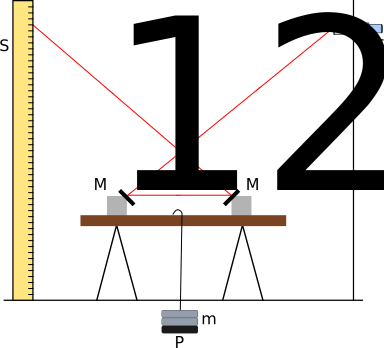
\includegraphics[scale=0.7]{koenig-setup.pdf}
			\caption{The experimental setup}
		\end{figure}
		The experimental arrangement is as shown in the figure. The bar is mounted on a knife edge which carries the load on a pan P. At the ends of the bar two mirrors $M_1$ and $M_2$, almost normal to the bar, but slightly displaced, are fixed to enable a scale S to be seen in the telescope T, the light from S having suffered $2$ reflections. 
		
		The telescope carries a crosswire in the eye-piece and the apparatus is arranged so that scale divisions as seen in the telescope coincides with crosswire. If now the bar is loaded with say $0.5$ or $1$ {kg}, as a result of the depression produced, the scale division viewed in the telescope will be altered by the particular divisions. One can determine the Young's modulus using the relation: 
		
		\begin{equation}
		Y=\dfrac{3WL^2(2D+\alpha)}{2bd^3x}
		\end{equation}
		where,  	
		\begin{eqnarray*}
			W &=& mg \text{ where m is load in kg} \\
			l &\rightarrow& \text{ distance between the knife edges in m}\\ 
			D &\rightarrow& \text{ distance between scale and the more remote mirror M$_2$ in m}\\
			\alpha &\rightarrow& \text{distance between the mirrors in m} \\ 
			b &\rightarrow& \text{breadth of the bar in m}\\
			d &\rightarrow& \text{ Thickness of the bar in m}
		\end{eqnarray*}
	
	\section{PROCEDURE}
		\begin{enumerate}
			\item Arrange the apparatus as shown in figure.
			\item Adjust the telescope to get a clear image of the scale on the mirror $M_1$.
			\item Place the $0.5$ kg load in the pan bar and take the scale readings which coincides with crosswire. Note the value.
			\item Repeat the above step by adding equal loads upto $3.5$ kg and note the corresponding depression.
			\item Find the values of $l$, $D$ and $\alpha$ using a meter scale, and values of $b$ and $d$ using a screw gauge.
			\item Plot a graph of load versus depression. The slope of the graph gives the value of $\left(\dfrac{m}{x}\right)$. Substituting it in the equation, $Y$ can be obtained.
		\end{enumerate}
		
	\section{OBSERVATIONS}
		\begin{center}
			\begin{tabular}{|c|c|c|c|c|c|}
			\hline
			\rowcolor{b1!50}&& \multicolumn{3}{c|}{Reading of scale in mirror (cm)} & \\
			\rowcolor{b1!50}\cline{3-5}
			\rowcolor{b1!50}Sl.no.& Load&&&& Depression\\
			\rowcolor{b1!50}& $m$&Load increase&Load decrease&Average&$x$\\
			\rowcolor{b1!50}& (kg) &&&&(cm)\\
			\hline
			&&&&&\\&&&&&\\&&&&&\\&&&&&\\&&&&&\\&&&&&\\
			\hline
		\end{tabular}
		\end{center} 	
			\vspace{10pt}
			Distance between the knife edged, l = \rule{10ex}{0.2pt}\\
			Distance between scale and the mirror, $M_2$ =\rule{10ex}{0.2pt}\\
			Distance between mirrors, $\alpha$ = \rule{10ex}{0.2pt}\\
			Breadth of the bar, $b$ =\rule{10ex}{0.2pt}\\
			Thickness of the bar, $d$ =\rule{10ex}{0.2pt}\\
			
		\section{CALCULATIONS}
			
			The plot of load versus depression gives a straight line. The slope of this line is given by
			
			$$\text{slope}=\dfrac{\Delta x}{\Delta m}$$
			
			\begin{figure}[!htb]
				\centering
				\includegraphics[scale=1]{koenig-graph.png}
			\end{figure}
			
			From equation (1),
			
			$$Y = \dfrac{3Wl^2(2D+\alpha)}{2bd^3x} = \dfrac{3mgl^2(2D+\alpha)}{2bd^3x}$$
			
			$$\therefore Y = \dfrac{3gl^{2}\left(2D+\alpha\right)}{2bd^{3}x} \left(\dfrac{m}{x}\right)$$
			
			$$\Rightarrow Y=\dfrac{3gl^{2}\left(2D+\alpha\right)}{2bd^{3}x} \left(\dfrac{1}{\text{slope}}\right)$$
			
	
	\section{RESULT}
		The Young's modulus of the bar is \rule{20ex}{0.2pt}$Pa$.
			
\end{document}